% gc-08-Applications.tex

\documentclass[xcolor=dvipsnames]{beamer}
\usepackage{teachbeamer}

\title{Applications of Derivatives}
\subtitle{{\CourseNumber}, BCIT}

\author{\CourseName}

\date{January 30, 2018}

% \begin{figure}[h]
% 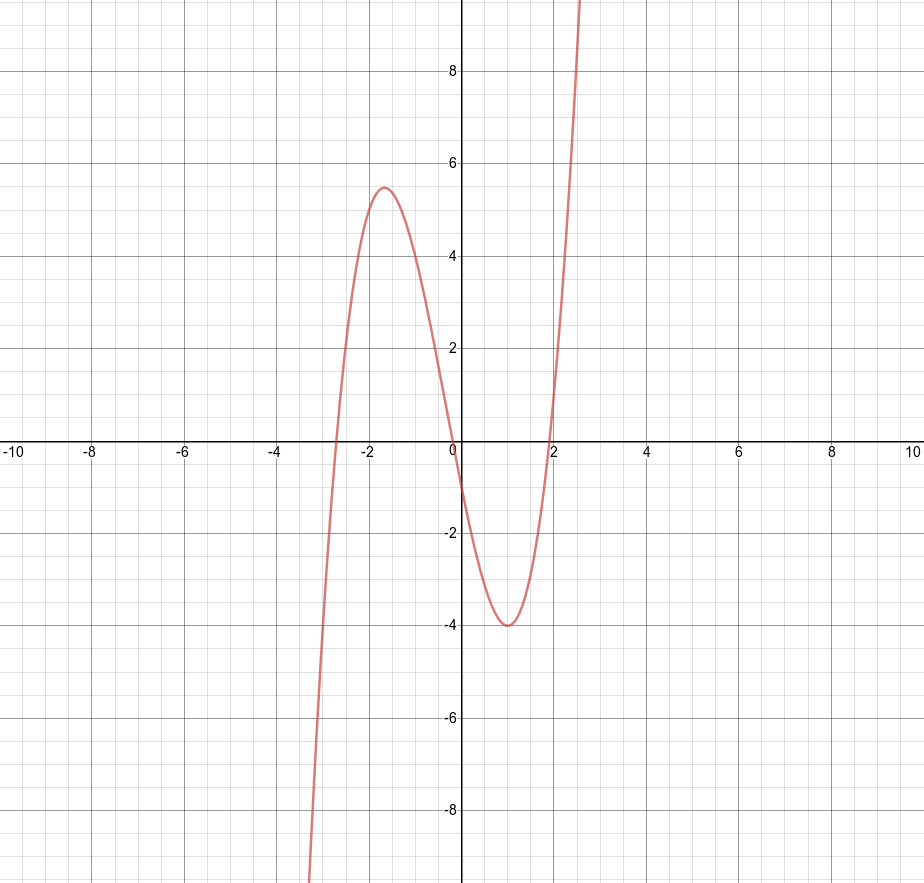
\includegraphics[scale=.3]{./diagrams/extrema1.png}
% \end{figure}

\begin{document}

\begin{frame}
  \titlepage
\end{frame}

\begin{frame}
  \frametitle{Rate of Change}
If $f(t)$ expresses some type of position of something dependent on
time $t$, then the rate of change over an interval is the slope of the
secant line. The derivative $f'(t)$ is then the instantaneous rate of
change or the slope of the tangent line at $t$. 

\bigskip

Sometimes the rate of change is not with respect to a position. For
example, acceleration is the rate of change with respect to a
velocity. Another common example is the rate of change in numbers of a
population. In economics, the rate of change in pricing may be of
interest.
\end{frame}

\begin{frame}
  \frametitle{Exercises for Rate of Change (Position)}
% James Stewart, Single Variable Calculus, Early Transcendentals, 6E,
% page 8
If a ball is given a push so that it has an initial velocity of $5$m/s
down a certain inclined plane, then the distance it has rolled after
$t$ seconds is $s=5t+3t^{2}$.
  \begin{enumerate}
  \item<1-> Find the velocity after 2 seconds.
  \item<2-> How long does it take for the velocity to reach 35m/s?
  \end{enumerate}
\end{frame}

\begin{frame}
  \frametitle{Exercises for Rate of Change (Position)}
% James Stewart, Single Variable Calculus, Early Transcendentals, 6E,
% page 8
Define $f(t)=5t+3t^{2}$. The derivative is $v(t)=f'(t)=5+6t$. Locate
the time at which $v(t)=5$ by solving the equation $5=5+6t$. The
initial time is $t=0$. Then
\begin{equation}
  \label{eq:airaiwie}
  v(2)=f'(2)=5+6\cdot{}2=17
\end{equation}
The velocity after 2 seconds is 17m/s.
\begin{equation}
  \label{eq:zeidieba}
  v(t)=35=5+6t\hspace{.5in}\Rightarrow\hspace{.5in}t=5
\end{equation}
The velocity after 5 seconds is 35m/s.
\end{frame}

\begin{frame}
  \frametitle{Exercises for Rate of Change (Geometry)}
% James Stewart, Single Variable Calculus, Early Transcendentals, 6E,
% page 8
A stone is dropped into a lake, creating a circular ripple that
travels outward at a speed of 60cm/s. Find the rate at which the area
within the circle is increasing after one second; three seconds; and
five seconds. What can you conclude?
\end{frame}

\begin{frame}
  \frametitle{Exercises for Rate of Change (Geometry)}
% James Stewart, Single Variable Calculus, Early Transcendentals, 6E,
% page 8
  Define a function for the radius dependent on time.
  \begin{equation}
    \label{eq:zoozohte}
    r(t)=60t
  \end{equation}
  Define a function for the area of the circle dependent on time.
  \begin{equation}
    \label{eq:maeneong}
    A(t)=\pi(r(t))^{2}=\pi(60t)^{2}=3600\pi{}t^{2}
  \end{equation}
  Differentiate
  \begin{equation}
    \label{eq:cheemahv}
    A'(t)=7200\pi{}t
  \end{equation}
  The circle of the area increases by $7200\pi$cm$^{2}$ per second
  after one second; by $21600\pi$cm$^{2}$ per second after three
  seconds; by $36000\pi$cm$^{2}$ per second after five seconds.
\end{frame}

\begin{frame}
  \frametitle{Exercises for Rate of Change (Physics)}
% James Stewart, Single Variable Calculus, Early Transcendentals, 6E,
% page 8
Newton's Law of Gravitation says that the magnitude $F$ of the force
exerted by a body of mass $m$ on a body of mass $M$ is 
\begin{equation}
  \label{eq:zeipouqu}
  F=\frac{GmM}{r^{2}}
\end{equation}
where $G$ is the gravitational constant and $r$ is the distance
between the bodies. Suppose it is known that the Earth attracts an
object with a force that decreases at the rate of 2N/km when
$r=20,000$km (N=kg$\cdot$m/s$^{2}$). What is the mass of the object?
Assume the following as constants:
% \begin{tabular}{|l|rcl|}\hline
%   gravitational constant & $G$&=&$6.67408\cdot{}10^{−11}\mbox{m}^{3}\mbox{kg}^{−1}\mbox{s}^{−2}$ \\ \hline
%   mass of the Earth & $m$&=&$5.9722\cdot{}10^{24}\mbox{kg}$ \\ \hline
% \end{tabular}
\begin{equation}
  \label{eq:phosulee}
  % G=6.67408\cdot{}10^{−11}\mbox{m}^{3}\mbox{kg}^{−1}\mbox{s}^{−2}
  G=6.67408\cdot{}10^{-11}m^{3}kg^{-1}s^{-2}
\end{equation}
\begin{equation}
  \label{eq:otienaix}
  % m=5.9722\cdot{}10^{24}\mbox{kg}
  m=5.9722\cdot{}10^{24}kg
\end{equation}
\end{frame}

\begin{frame}
  \frametitle{Exercises for Rate of Change (Population)}
% James Stewart, Single Variable Calculus, Early Transcendentals, 6E,
% page 9
The number of yeast cells in a laboratory culture increases rapidly
initially but levels off eventually. The population is modeled by the
function
\begin{equation}
  \label{eq:kupeivae}
  n=f(t)=\frac{a}{1+be^{-0.7t}}
\end{equation}
where $t$ is measured in hours. At time $t=0$ the population is 20
cells and is increasing at a rate of 12 cells per hour. Find the
values of $a$ and $b$. According to this model, what happens to the
yeast population in the long run?
\end{frame}

\begin{frame}
  \frametitle{Exercises for Rate of Change (Economics)}
% James Stewart, Single Variable Calculus, Early Transcendentals, 6E,
% page 9
The cost, in dollars, of producing $x$ yards of a certain fabric is
\begin{equation}
  \label{eq:uquuthae}
  C(x)=1200+12x-0.1x^{2}+0.0005x^{3}
\end{equation}
\begin{enumerate}
\item<1-> Find the marginal cost function.
\item<2-> Find $C'(200)$ and explain its meaning. What does it
  predict?
\item<3-> Compare $C'(200)$ with the cost of manufacturing the 201st
  yard of fabric.
\end{enumerate}
\end{frame}

\begin{frame}
  \frametitle{Exponential Growth and Decay I}
  Growth often happens proportional to size. For example, a population
  of 500 will grow to 550 during a given period of time while at the
  same growth rate a population of 1000 will grow to 1100 during the
  same period of time. Interest on a bank account is another example.
  Radioactive decay is an example for decay, sometimes also called
  negative growth. 

\bigskip

The growth rate $f'(t)$ should be proportional to the population
$f(t)$, so $f'(t)=kf(t)$, where $k$ is some constant. We already know
that the function
\begin{equation}
  \label{eq:sohngiel}
  f(t)=Ce^{kt}
\end{equation}
fulfills this constraint. It turns out that the function in
(\ref{eq:sohngiel}) is the only function fulfilling this constraint.
Calculate $C$ in terms of $f$.
\end{frame}

\begin{frame}
  \frametitle{Exponential Growth and Decay II}
Many natural phenomena have been found to follow the law that an
amount $f(t)$ varies with time $t$ according to
  \begin{equation}
    \label{eq:lauwutho}
    f(t)=f(0)e^{kt}
  \end{equation}
If $k>0$, there is growth. If $k<0$, there is decay.
\end{frame}

\begin{frame}
  \frametitle{Uninhibited Growth and Decay Exercise}
A colony of bacteria grows according to the law of uninhibited growth
according to the function
\begin{equation}
  \label{eq:chiowezo}
  N(t)=100e^{0.045t}
\end{equation}
where $N$ is measured in grams and $t$ is measured in days.
  \begin{enumerate}
  \item<1-> Determine the initial amount of bacteria.
  \item<2-> What is the growth rate of the bacteria?
  \item<3-> What is the population after five days?
  \item<4-> How long will it take for the population to reach 140
    grams?
  \item<5-> What is the doubling time for the population?
  \end{enumerate}
\end{frame}

\begin{frame}
  \frametitle{Radiocarbon Dating}
Radiocarbon dating is a method archeologists use to determine the age
of ancient objects. The carbon dioxide in the atmosphere always
contains a fixed fraction of radioactive carbon, carbon-14 ($^{14}$C),
with a half-life of about 5730 years. Plants absorb carbon dioxide
from the atmosphere, which then makes its way to animals through the
food chain. Thus, all living creatures contain the same fixed
proportions of $^{14}$C to nonradioactive $^{12}$C as the atmosphere.

\medskip

After an organism dies, it stops assimilating $^{14}$C, and the amount
of $^{14}$C in it begins to decay exponentially. We can then determine
the time elapsed since the death of the organism by measuring the
amount of $^{14}$C left in it.
\end{frame}

\begin{frame}
  \frametitle{Radiocarbon Dating Example}
If a donkey bone contains 73\% as much $^{14}$C as a living donkey,
when did it die?

\medskip

Look at the following table to notice the pattern,
\begin{equation}
  \label{eq:sayeeziu}
  \begin{array}{rcccl}
        100\% & \ldots & 2^{-0} & \ldots & 5730\cdot{}0 \\
        50\% & \ldots & 2^{-1} & \ldots & 5730\cdot{}1 \\
        25\% & \ldots & 2^{-2} & \ldots & 5730\cdot{}2
  \end{array}
\end{equation}
Therefore ($t$ being the number of years ago that the donkey died),
\begin{equation}
  \label{eq:anuvuama}
  t=\left(-\log_{2}0.73\right)\cdot{}5730=-\frac{\ln{}0.73}{\ln{}2}\cdot{}5730\approx{}2600
\end{equation}
\end{frame}

\begin{frame}
  \frametitle{Radioactive Decay}
The half-life of radium-226 is 1590 years. A sample of radium-226 has
a mass of 100mg. 
\begin{enumerate}
\item<1-> Find a formula for the mass of the sample that
remains after $t$ years.
\item<2-> Find the mass ofter 1000 years correct to the nearest
  milligram.
\item<3-> When will the mass be reduced to 30 mg?
\end{enumerate}
\end{frame}

\begin{frame}
  \frametitle{Newton's Law of Cooling}
The temperature $u$ of a heated object at a given time $t$ can be
modeled by the following function,
\begin{equation}
  \label{eq:iemahbec}
  u(t)=T+(u_{0}-T)e^{kt}
\end{equation}
where $k$ is a negative constant, $T$ is the constant temperature of
the surrounding medium, and $u_{0}$ is the initial temperature of the
heated object.
\end{frame}

\begin{frame}
  \frametitle{Newton's Law of Cooling Exercise 1}
An object is heated to 100$^{\circ}C$ (degrees Celsius) and is then
allowed to cool in a room whose air temperature is 30$^{\circ}C$.
\begin{enumerate}
\item<1-> If the temperature of the object is $80^{\circ}C$ after five
  minutes, when will its temperature be $50^{\circ}C$?
\item<2-> Determine the elapsed time before the temperature of the
  object is $35^{\circ}C$.
\item<3-> What do you notice about $u(t)$, the temperature, as $t$,
  time, passes?
\end{enumerate}
\end{frame}

\begin{frame}
  \frametitle{Newton's Law of Cooling Exercise 2}
A frozen steak has a temperature of $28^{\circ}F$. It is placed in a
room with a constant temperature of $70^{\circ}F$. After 10 minutes,
the temperature of the steak has risen to $35^{\circ}F$. 
\begin{enumerate}
\item<1-> What will the temperature of the steak be after 30 minutes?
\item<2-> How long will it take the steak to thaw to a temperature of $45^{\circ}F$?
\end{enumerate}
\end{frame}

\begin{frame}
  \frametitle{Newton's Law of Cooling Exercise 3}
The hotel Bora-Bora is having a pig roast. At noon, the chef put the
pig in a large earthen oven. The pig's original temperature was
$75^{\circ}F$. At 2:00\textsc{pm} the chef checked the pig's
temperature and was upset because it had reached only $100^{\circ}F$.
\begin{enumerate}
\item If the oven's temperature remains a constant $325^{\circ}F$, at
  what time may the hotel serve its guests, assuming that pork is done
  when it reaches $175^{\circ}F$?
\end{enumerate}
\end{frame}

\begin{frame}
  \frametitle{Newton's Law of Cooling Exercise 4}
  Suppose that a corpse was discovered in a motel room at midnight and
  its temperature was $80^{\circ}F$. The temperature of the room is
  kept constant at $60^{\circ}F$. Two hours later the temperature of
  the corpse dropped to $75^{\circ}$. Find the time of death (i.e.\
  the time when the temperature of the body was 98.6$^{\circ}F$).
  Round the time to the nearest minute.
\end{frame}

\begin{frame}
  \frametitle{End of Lesson}
Next Lesson: Maxima and Minima
\end{frame}

\end{document}

